% !TeX program = lualatex -synctex=1 -interaction=nonstopmode --shell-escape %.tex
\documentclass[_Venture_p3.tex]{subfiles}

\begin{document}

\setbeamercovered{invisible}

\subsection{Отрасль нанотехнологий}
\begin{frame}{Отрасль нанотехнологий}{Открытие фуллерена}
\begin{figure}
	\centering
	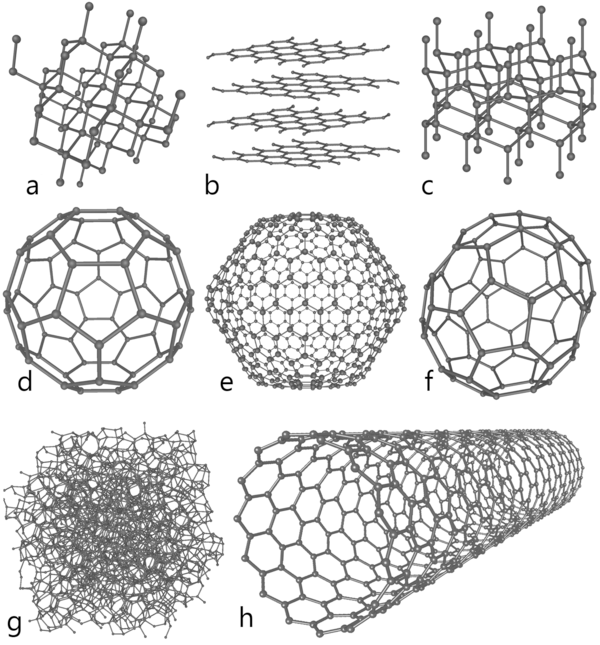
\includegraphics[%width=250pt,
	height=150pt,
	keepaspectratio=true,]
	{img/carbon_nanotube.png}
	\caption{\scriptsize{Формы углерода: a) алмаз, b) графит, c) метеоритный алмаз, d) фуллерен, e) фуллерит f) фуллерен, g) уголь h) однослойная углеродная нанотрубка}}
\end{figure}
\end{frame}

\begin{frame}{Наномасштаб}
\begin{block}{Наночастицы}
\quad - это частицы, одно из измерений которых меньше 100 нм.
\end{block}
\end{frame}


\newcolumntype{b}{>{\hsize=2.3\hsize}X}
\newcolumntype{s}{>{\hsize=.45\hsize}X}
\newcolumntype{m}{>{\hsize=.9\hsize}X}

\begin{frame}[shrink=15]
% Table generated by Excel2LaTeX from sheet 'Лист1'
\begin{table}
	\centering
	\caption{\captionf{Наномасштаб}}
	\begin{tabularx}{\linewidth}[b]{@{}>{\raggedright\arraybackslash}Xr@{}}
		\setrulecolor\toprule
		\cnamef{Объект} & \cnamef{Размер, м}\\\midrule 
		Ядро урана (диаметр) & $10^{-13}$ \\
		Молекула воды & $10^{-10}$ \\
		Молекула ДНК (ширина) & $10^{-9}$ \\
		\noindent\parbox[b]{\hsize}{\raggedright Протозоа (простейший \linebreak одноклеточный организм)} & $10^{-5}$ \\
		Дождевой червь & $10^{-2}$ \\
		Человек & 2 \\
		Эверест (высота) & $10^{4}$ \\
		Земля (диаметр) & $10^{8}$ \\
		\noindent\parbox[b]{\hsize}{\raggedright Солнечная система\linebreak (расстояние от Солнца до Плутона)} & $10^{13}$ \\
		\bottomrule
	\end{tabularx}%
	\label{tab:addlabel}%
\end{table}%
\end{frame}

\begin{frame}{Наноинструменты}
\begin{itemize}
	\item сканирующий   электронный   микроскоп   (scanning electron microscope), или СЭМ (SEM);
	\item просвечивающий электронный микроскоп (transmission electron microscope), или ПЭМ (ТЕМ);
	\item аналитический электронный микроскоп (analytical electron microscope), или АЭМ (АЕМ).
\end{itemize}
\end{frame}

\begin{frame}
\begin{figure}
	\centering
	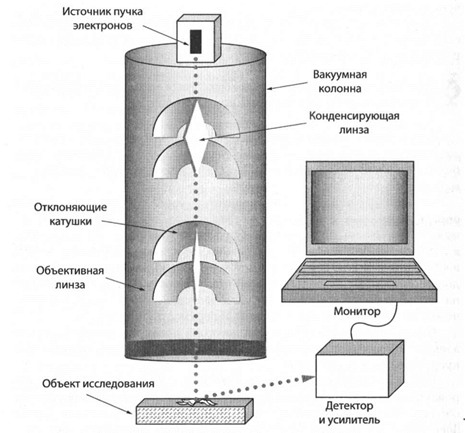
\includegraphics[scale=.6]{img/electronic_microscope}
	\caption{Принцип работы электронного микроскопа}
\end{figure}
\end{frame}

\begin{frame}
\begin{figure}
	\centering
	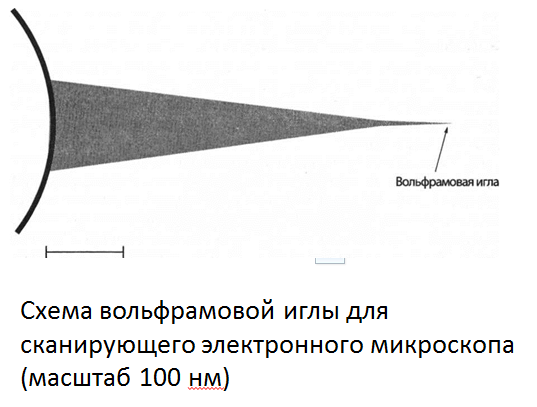
\includegraphics[scale=.7]{img/nanomanipulator}
	\caption{Наноманипуляторы}
\end{figure}
\end{frame}

\begin{frame}
СЗМ с компьютерным управлением позволяет в оперативном режиме манипулировать наночастицами. 

Некоторые системы для наноманипулирования имеют виртуальный интерфейс пользователя, который напоминает игру с элементами виртуальной реальности.
\end{frame}

\begin{frame}{Оптические пинцеты }
предоставляют еще один способ захвата и перемещения нанометровых структур в трехмерном пространстве. 

Эта возможность особенно важна при изучении динамики атомов и молекул, поскольку специалистам молекулярной биофизики важно понимать поведение отдельных молекул.

\end{frame}

\subsection{Органические приложения нанотехнологий}
\begin{frame}
\begin{block}{Наномедицина}
	\quad — это область медицины, в которой лечение болезней и операции выполняются на молекулярном уровне.
\end{block}
\begin{itemize}
	\item раннее обнаружение и устранение раковых клеток;
	\item удаление или замена испорченных компонентов клетки с помощью наномасштабных устройств;
	\item создание и имплантация молекулярных насосов для доставки медикаментов.
\end{itemize}
\end{frame}

\begin{frame}[allowframebreaks]{Нанотехнологи для решения медицинских задач}
\begin{itemize}
	\item хранения и извлечения генетической информации;
	\item диагностики, например обнаружения болезни;
	\item определения общей восприимчивости к некоторым болезням, например к болезни Альцгеймера;
	\item улучшенной классификации болезней, например разбивки их на типы и подтипы;
	
	\pagebreak
	\item точечного подбора лекарств на основе хромосомных различий;
	\item генной терапии, например для кистозного фиброза;
	\item подбора медикаментов, нацеленных на отдельные клетки, например, создания антител для специальных клеток.
\end{itemize}
\end{frame}

\begin{frame}
\begin{figure}
	\centering
	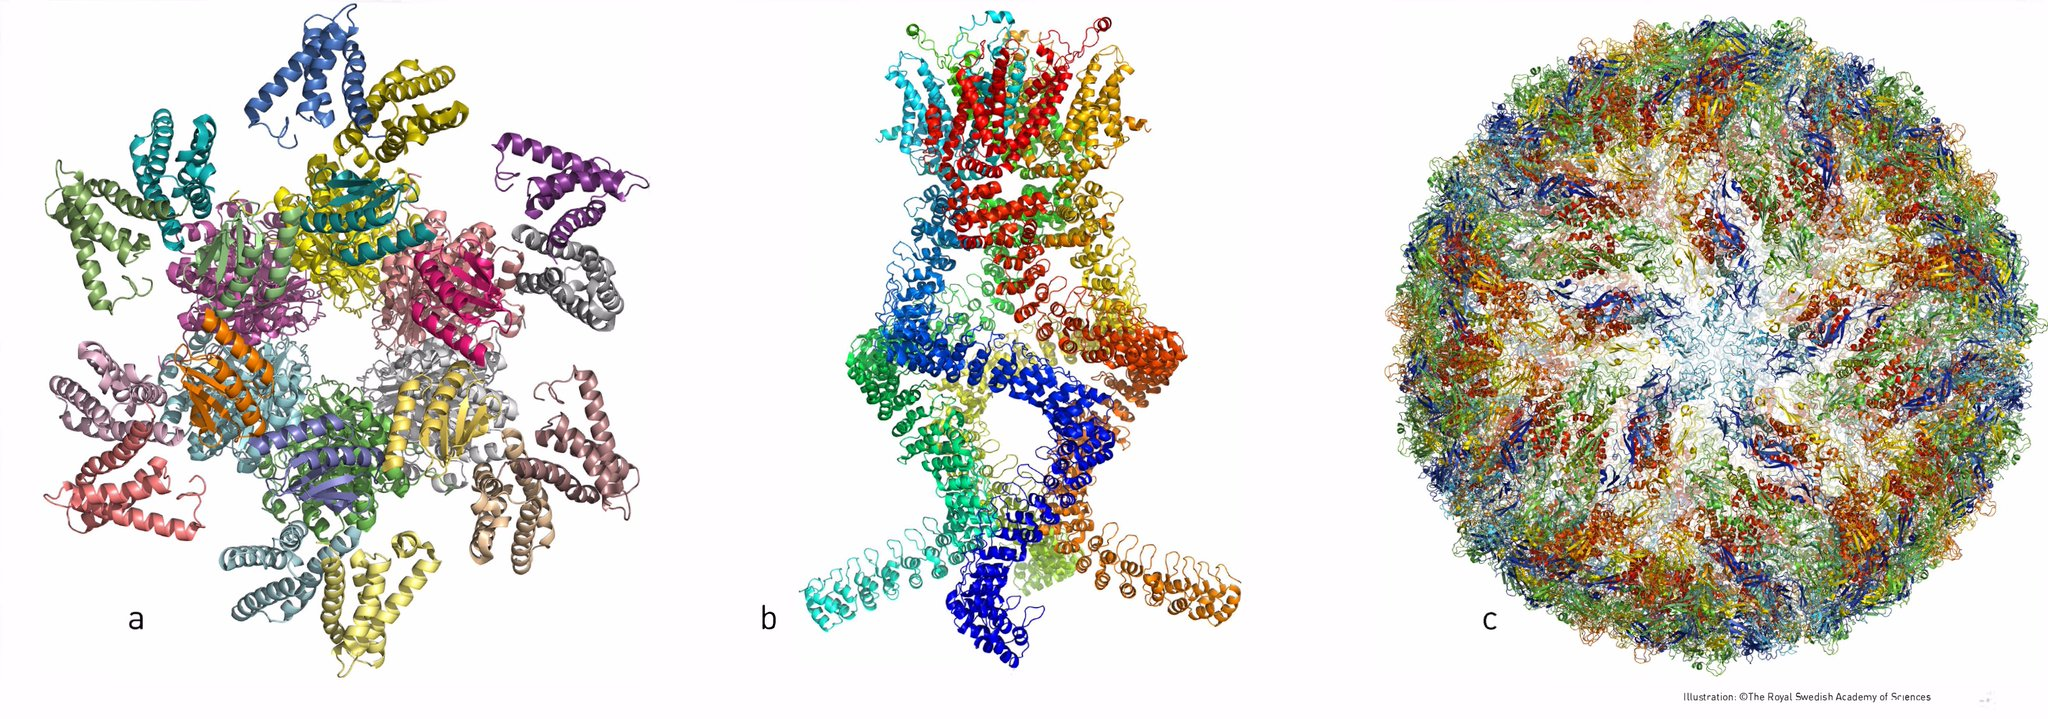
\includegraphics[scale=.2]{img/proteins_atomic_structures}
	\caption{Атомная структура a) белка, отвечающего за ``биологические часы``; b) измерителя давления, который задействован в органах слуха; c) вируса Зика }
\end{figure}
Криоэлектронная микроскопия, Нобелевская премия по химии 2017г.
\end{frame}


\begin{frame}
\begin{figure}
	\centering
	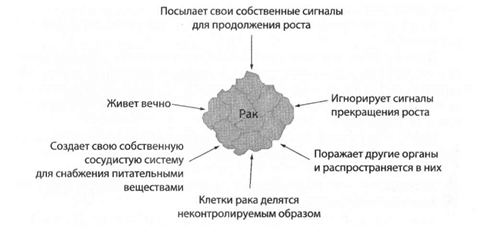
\includegraphics[scale=.95]{img/cancer_characteristics}
	\caption{Способы проникновения рака в тело человека}
\end{figure}
\end{frame}

\begin{frame}{Виды нанотехнологий}{применяемых в медицине}
\begin{itemize}
	\item лаборатория-на-чипе;
	\item кремниевые нанопровода;
	\item золотые нанооболочки;
	\item сварка тканей;
	\item оптическая когерентная томография;
	\item доставка медикаментов.
\end{itemize}
\end{frame}

\begin{frame}{Применение золотых нанооболочек в медицине}{Лечение рака}
\begin{figure}
	\centering
	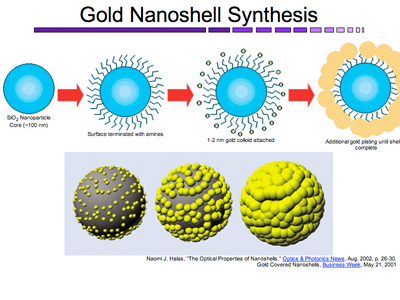
\includegraphics[scale=.7]{img/nanoshells}
	\caption{Золотые нанооболочки являются простыми, но очень эффективными наноагентами}
\end{figure}
\end{frame}

\begin{frame}{Применение золотых нанооболочек в медицине}{Лечение рака}
\begin{figure}
	\centering
	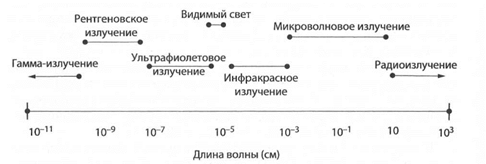
\includegraphics[scale=.7]{img/wave_lenghts}
	\caption{Шкала длин волн и энергий электромагнитного излучения}
\end{figure}
\end{frame}

\begin{frame}
\begin{figure}
	\centering
	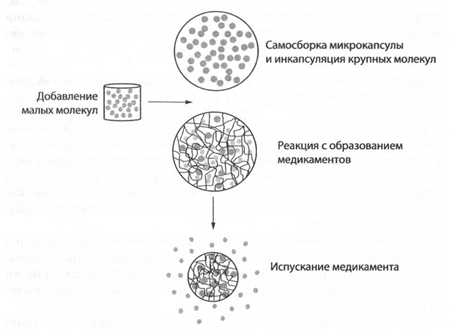
\includegraphics[scale=.7]{img/microcapsule}
	\caption{Самособирающиеся микрокапсулы дают возможность доставлять медикаменты в нужное место в организме человека}
\end{figure}
\end{frame}

\begin{frame}
\begin{figure}
	\centering
	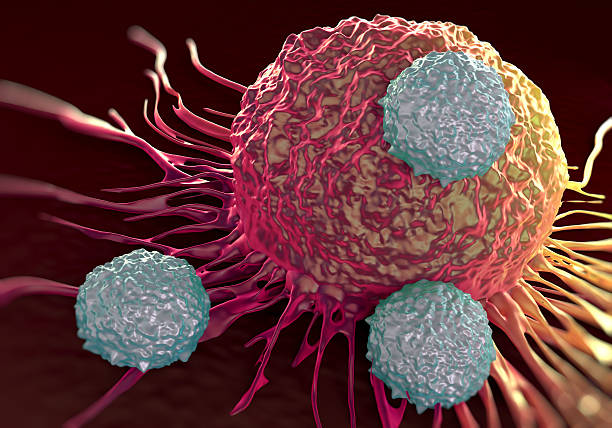
\includegraphics[scale=.45]{img/tcell_attacking_cancer_cell}
	\caption{Иммунная клетка человека (белая) атакует раковую клетку.}
\end{figure}
\end{frame}

\subsection{Нанотехнологии и охрана окружающей среды}
\begin{frame}{Нанотехнологии и охрана окружающей среды}{Наиболее распространенные загрязняющие вещества}
\begin{itemize}
	\item окись углерода (или угарный газ);
	\item фреон (chlorofluorocarbon — CFC);
	\item тяжелые металлы (мышьяк, хром, кадмий, свинец, ртуть, цинк);
	\item углеводороды;
	\item оксиды азота;
	\item органические химикаты (летучие органические соединения, диоксины);
	\item диоксид серы (или сернистый ангидрид);
	\item макрочастицы.
\end{itemize}
\end{frame}

\begin{frame}{Нанотехнологии и охрана окружающей среды}
\begin{figure}
	\centering
	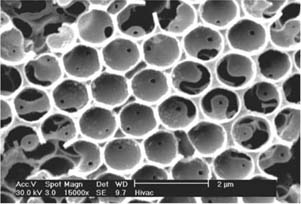
\includegraphics[scale=.7]{img/membrane_ferroxane}
	\caption{Мембрана из ферроксана (ferroxane) }
\end{figure}
Мембрана из керамики на основе оксида железа. 

Благодаря уникальным химическим свойствам железа эти реактивные мембраны позволяют очищать воду, удаляя из нее загрязняющие вещества и органические отходы.
\end{frame}

\begin{frame}
\begin{figure}
	\centering
	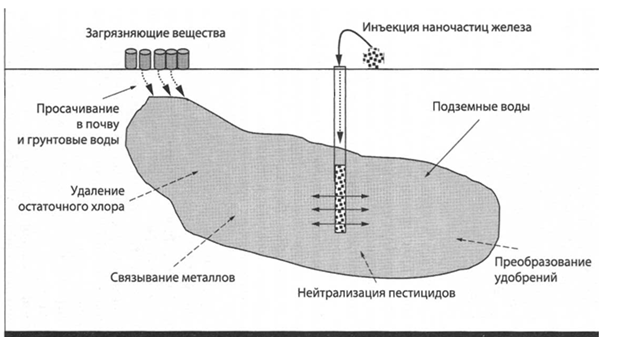
\includegraphics[scale=.7]{img/cleaning_environment}
	\caption{Очистка грунтовых вод с помощью инъекции наночастиц железа}
\end{figure}
\end{frame}

\begin{frame}
Железо обладает способностью легко окисляться и образовывать ржавчину. Если это окисление происходит в присутствии загрязняющих веществ, то их сложные молекулы распадаются на простые и менее токсичные углеродные компоненты.
\end{frame}

\subsection{Неорганические приложения нанотехнологий}
\begin{frame}{Неорганические приложения нанотехнологий}
Наноматериалы могут обладать чрезвычайно высокой прочностью, твердостью, гибкостью, вязкостью при высоких температурах, износостойкостью, коррозионной стойкостью, химической реактивностью и т. д.
\end{frame}

\begin{frame}{Применение умных материалов}
\begin{figure}	
	\centering
	\begin{subfigure}[t]{4.2cm}
		\centering
		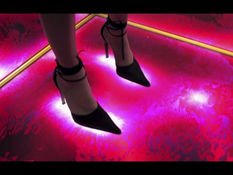
\includegraphics[scale=.95]{img/smart_materials_a.png}
		\caption{в архитектуре}\label{fig:a}	
	\end{subfigure}
	\quad
	\begin{subfigure}[t]{4.2cm}
		\centering
		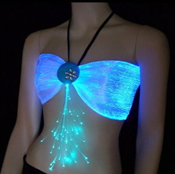
\includegraphics[scale=.95]{img/smart_materials_b.png}
		\caption{футуротекстиль}\label{fig:b}
	\end{subfigure}
	\caption{Умные материалы}\label{fig:smart_materials1}
\end{figure}
\end{frame}

\begin{frame}{Умные материалы}
\begin{figure}	
	\centering
	\begin{subfigure}[t]{4.2cm}
		\centering
		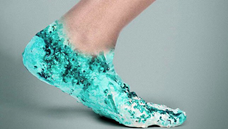
\includegraphics[scale=0.95]{img/smart_materials_c.png}
		\caption{4D печать}\label{fig:a}	
	\end{subfigure}
	\quad
	\begin{subfigure}[t]{4.2cm}
		\centering
		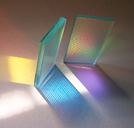
\includegraphics[scale=0.95]{img/smart_materials_d.png}
		\caption{строительство}\label{fig:b}
	\end{subfigure}
	\caption{Умные материалы}\label{fig:smart_materials1}
\end{figure}
\end{frame}

\begin{frame}{Квантовые точки}
Полупроводниковые наночастицы, которые способны захватывать электроны и локализовать их в малой области, называются квантовыми точками (quantum dots). 

Они способны испускать свет с разной длиной волны, в зависимости от собственного размера и уровней энергии. Применяются в качестве биологических маркеров, для обнаружения раковых опухолей с помощью флуоресцентной спектроскопии

\end{frame}

\begin{frame}{Нанокомпозиты}
- это новый класс материалов, который создается за счет введения наночастиц (наполнителя) в основной макроскопический материал (матрицу).

Например, некоторые нанокомпозиты создаются на основе внедрения наночастиц силикатной глины в пластмассы или керамику. Такие сверхтвердые нанокомпозиты уже используются в автомобильной промышленности для создания панелей и ступенек.

\end{frame}

\begin{frame}[allowframebreaks]{Производство микропроцессоров}
\begin{itemize}
	\item Литография — это технологический процесс репликации чертежа электросхемы на кремниевую подложку. 
	\item Чем короче длина волны, тем меньше вытравленные на подложке элементы (дорожки) электросхемы и выше плотность транзисторов.
	\item С помощью света с длиной волны 248 нм получается схема с дорожками шириной 200 нм.
	
	\pagebreak
	\item Современные кремниевые чипы создаются с помощью ультрафиолетового света с очень короткой длиной волны 20-40 нм. 
	\item Проводятся исследования экстремального ультрафиолетового света (extreme-ultraviolet lithography) с длиной волны около 10‑15 нм.
\end{itemize}
\end{frame}

\begin{frame}{Умные энергосети}
\begin{itemize}
	\item Наноматериалы, например углеродные нанотрубки, представляют собой один из вариантов, повышающих эффективность системы передачи электрической энергии. 
	
	\item Проводимость углеродных нанотрубок в 6 раз выше проводимости меди. 
	
	\item Углеродные нанотрубки они имеют меньший размер, что особенно важно в местах, где подземные коммуникации уже переполнены медными проводами.
\end{itemize}
\end{frame}

\begin{frame}
\begin{figure}
	\centering
	\begin{columns}
		\figurewithcaptionatside
		[caption position=b,caption on the right]
		{\caption{Космический лифт для доставки грузов на геостационарную орбиту}\label{fig:example right}}
		{\centering 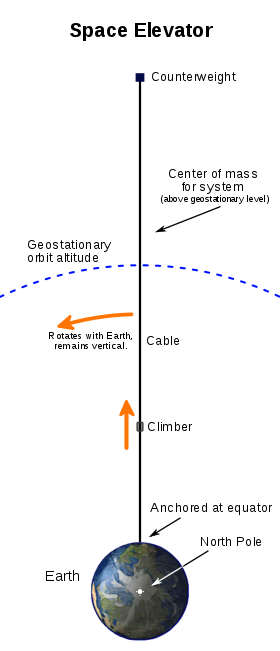
\includegraphics[scale=.50]{img/space_elevator}}
	\end{columns}
\end{figure}
\end{frame}
\subsection{Инвестиции в нанотехнологии}
\begin{frame}
\begin{figure}
	\centering
	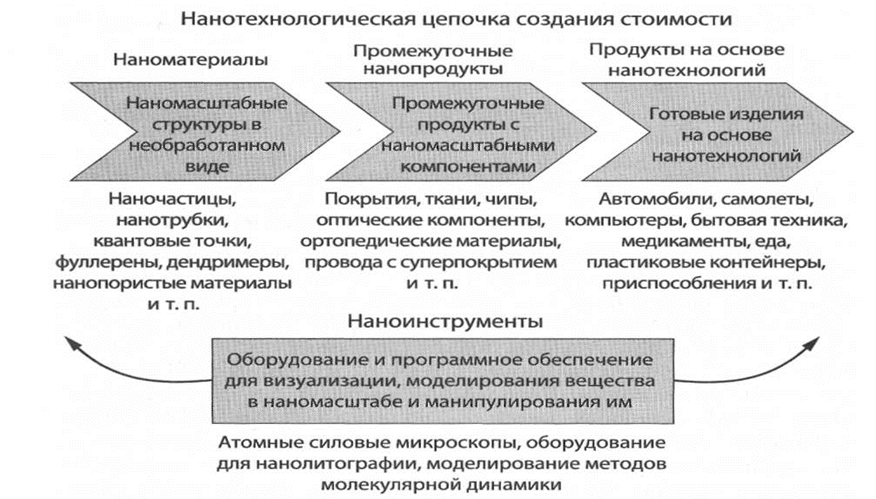
\includegraphics[scale=.45]{img/investment_in_nanotechnology}
	\caption{Создание стоимости в отрасли нанотехнологий.}
\end{figure}
\end{frame}
\end{document}